\chapter{Strategie 2}

(ZB)

Eine bekannte Wärmebehandlung von $\alpha$+$\beta$-Titanlegierungen ist die  \textit{Solution treatment and quenching + Aging}(Siehe Abbildung \ref{fig:SQ})). Im Gegensatz zu  Strategie 1, wird hier ein Duplex-Anneal zum Einstellen eines bimodalen Gefüges nicht gebraucht.(Diagramm WB Bild)  Werkstücke werden im ersten Schritt bei einer Temperatur unterhalb $T_{\beta}$ für 1--2 h geglüht und danach wassergekühlt. Vor Dem Abschrecken, stellt sich ein zweiphasiges Gefüge ein ($\alpha$ und $\beta$) (Verweis auf Gefügebild). Der große Beta-Anteil des Gefüges kann aber durch 2\% Molybdän auch nach einer vollständigen Diffusion nicht stabilisiert werden und wandelt beim Abschrecken martensitisch um. Dieses Gefüge wird dann $\alpha_p$--$\alpha^\prime$ genannt.
Dafür werden Ti-6242 Proben bei 983$^\circ$C für 60 min geglüht und dann wasserabgeschreckt. , da sich bei der Temperatur ein Gefüge mit ca. 84\% $\beta$ ein
Um das Gefüge noch weiter zu verfeinern, wird der zweite Wärmebehandlungsschritt das Anlassen durchgeführt. Hier sollen die Proben nochmal erwärmt  und dann luftgekühlt werden. bei der erhöhten Temperatur soll sich der Martensit in $\beta$ + $\alpha$ (Körner) umwandeln.
Um beide Strategien noch besser vergleichen zu können werden in diesem Schritt  die Proben bei  610$^\circ$C  für 30 min angelassen und danach luftgekühlt.

\begin{figure}[H]
	\centering
	{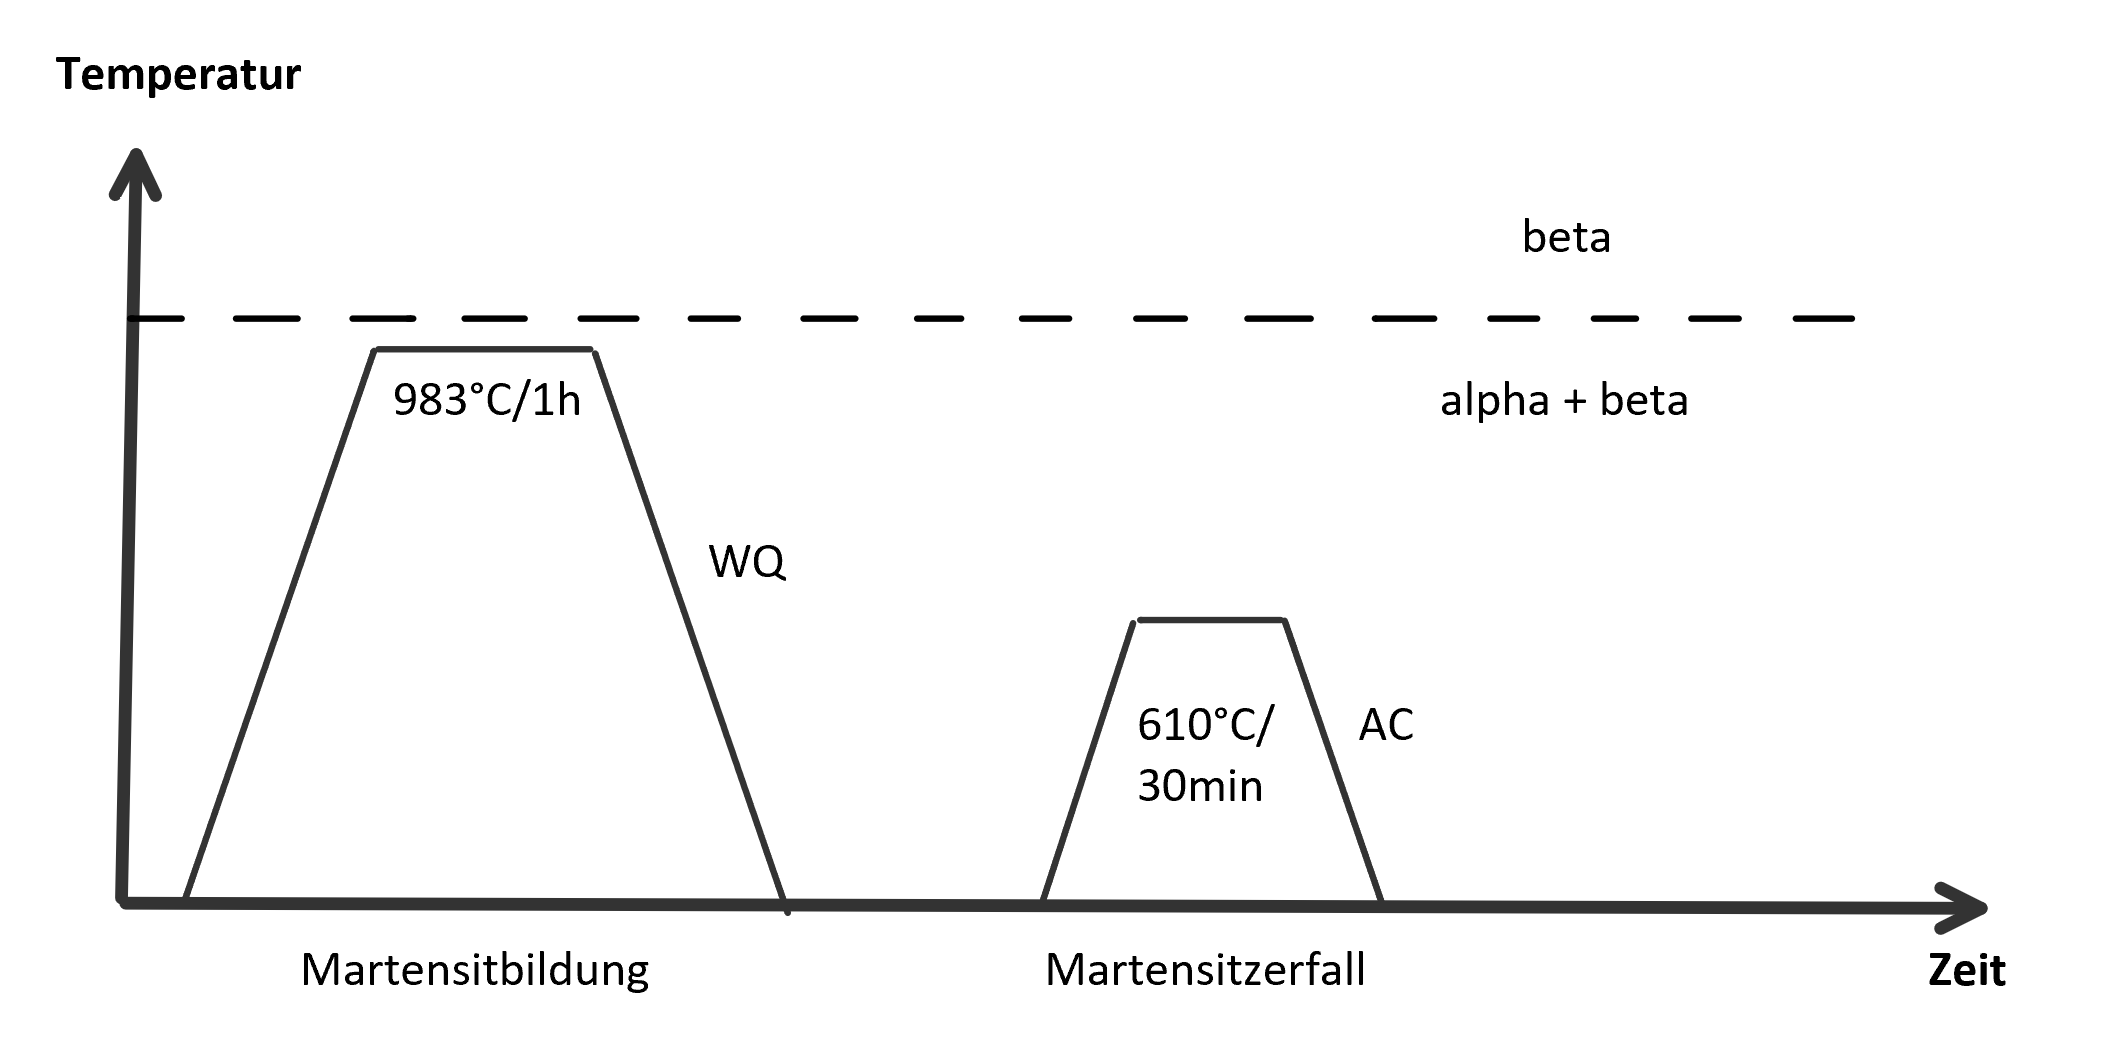
\includegraphics[width=0.9\textwidth]{./Bilder/SQ.png}}
	\caption{Wärmebehandlungsdiagramm von dem Solution Treatment and Quenching + aging}
	\label{fig:SQ}
\end{figure}

(PH)

Zum Vergleich wurde parallel eine $\alpha_p$ - $\alpha'$-Wärmebehandlung durchgeführt. Im Gegensatz zur der STDA-Wärmebehandlung, besitzt diese nur zwei Behandlungsschritte.
Dazu wurde wieder die aus der $\alpha_p$-Studie hervorgegangene Temperatur von 983$^\circ$C ausgewählt, eine Probe für 1 Stunde geglüht und anschließend wassergekühlt. Die dadurch entstandene Mikrostruktur wurde unter dem Lichtmikroskop ausgewertet und ist in Abbildung \ref{fig:abbildung-19} aufgeführt.

\begin{figure}
	\centering
	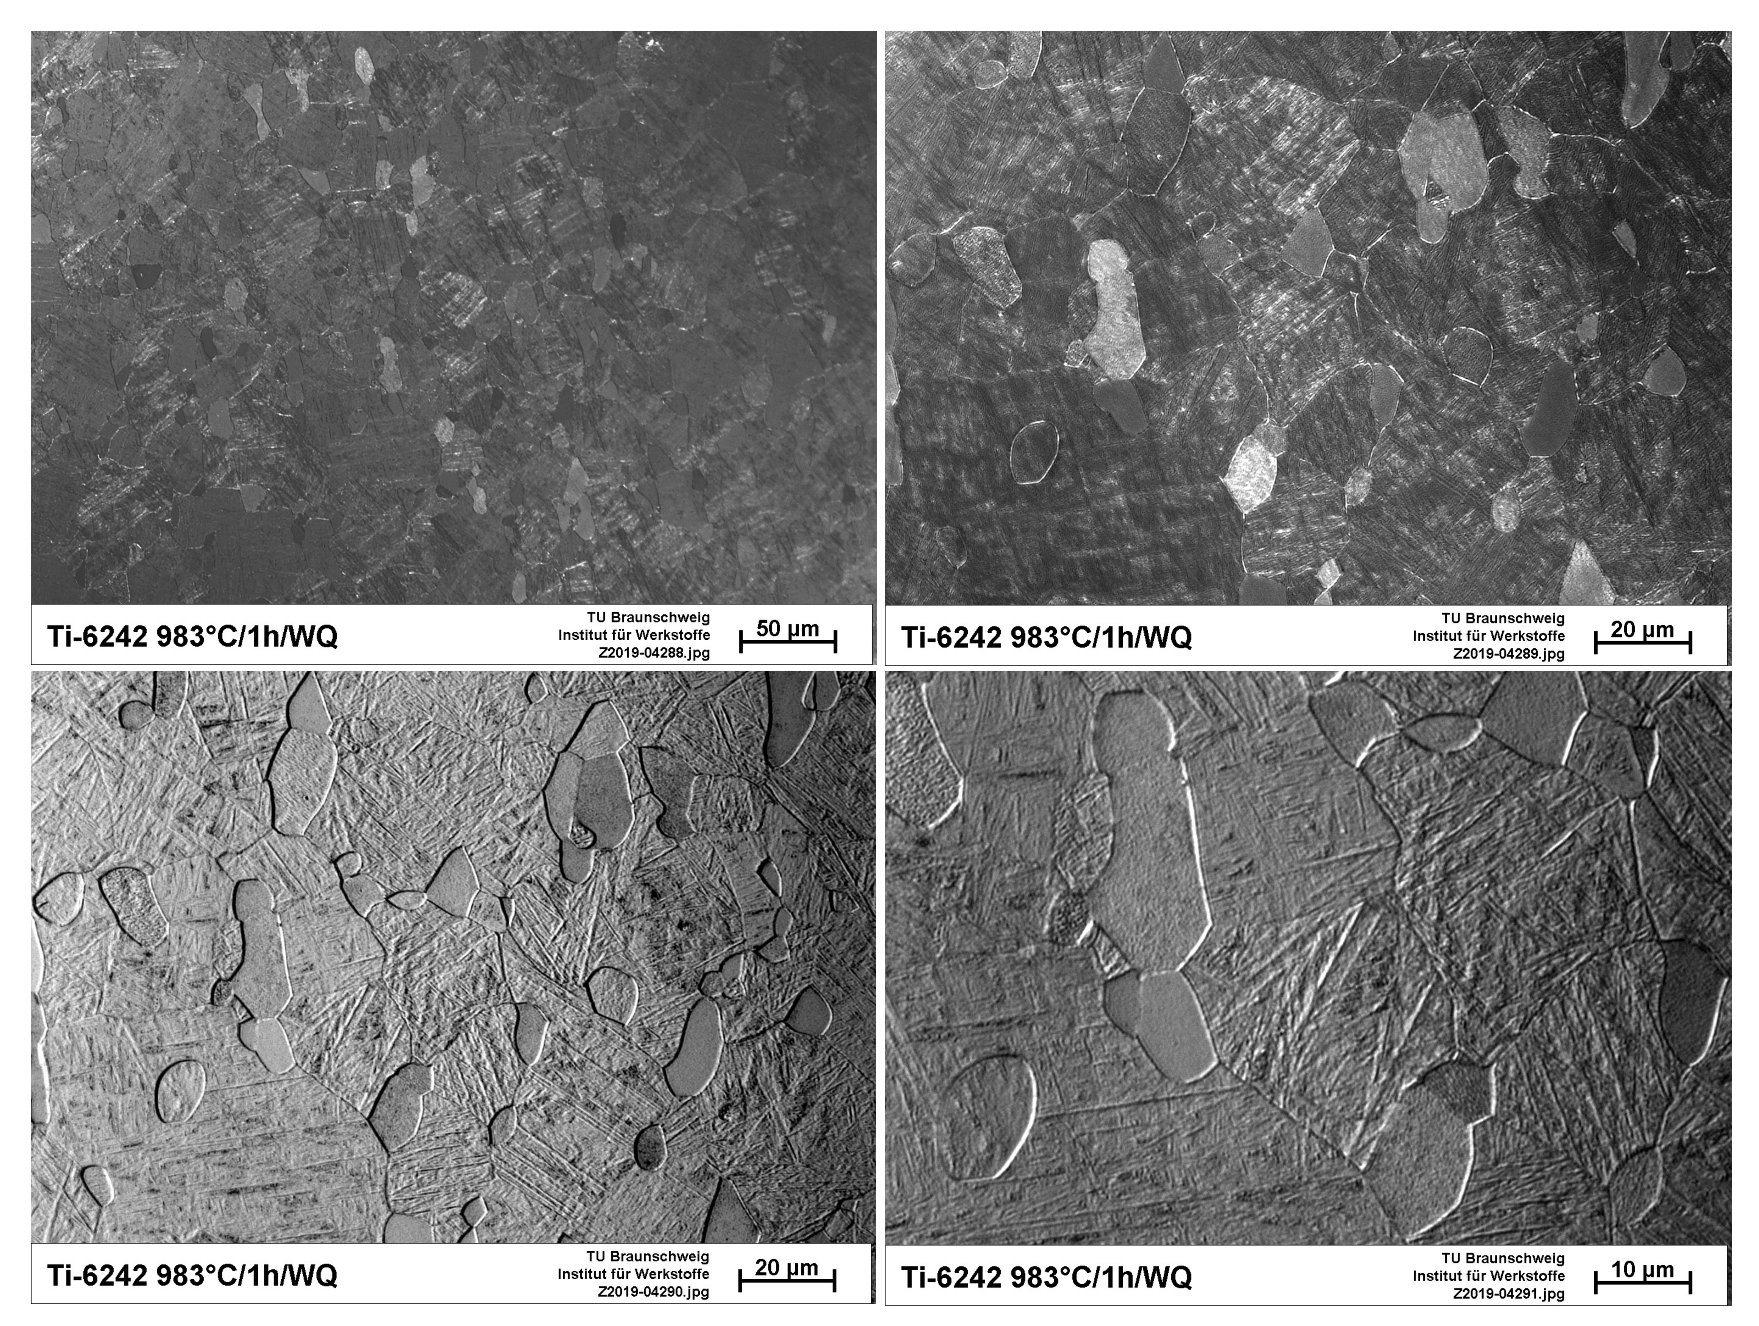
\includegraphics[width=1.0\linewidth]{./Bilder/Abbildung 19.png}
	\caption[Abbildung 19]{$\alpha_p$ - $\alpha'$-Gefüge unter dem Lichtmikroskop bei verschiedenen Vergrößerungen}
	\label{fig:abbildung-19}
\end{figure}

Der Unterschied in diesem ersten Schritt der Wärmebehandlung, im Vergleich zum ersten Schritt der STDA, liegt in der Wasserabkühlung. Das dadurch entstandene Gefüge besteht aus Primär-$\alpha$-Phase ($\alpha_p$) und Martensit ($\alpha'$), das als $\alpha_p$/$\alpha'$-Gefüge bezeichnet wird.

Die anschließende Härteprüfung ergab eine mittlere Vickershärte von 405 HV.

Im zweiten Schritt sollte wieder ein Martensitzerfall durchgeführt werden. Dazu wurden zwei Proben erneut bei 610$^\circ$C wärmebehandelt. Es wurden zwei Haltezeiten 16 und 30 min ausgewählt, mit anschließender Luftabkühlung. Die Auswertung unter dem REM ist in den Abbildungen \ref{fig:abbildung-26} und \ref{fig:abbildung-27} zusammengefasst.

\begin{figure}
	\centering
	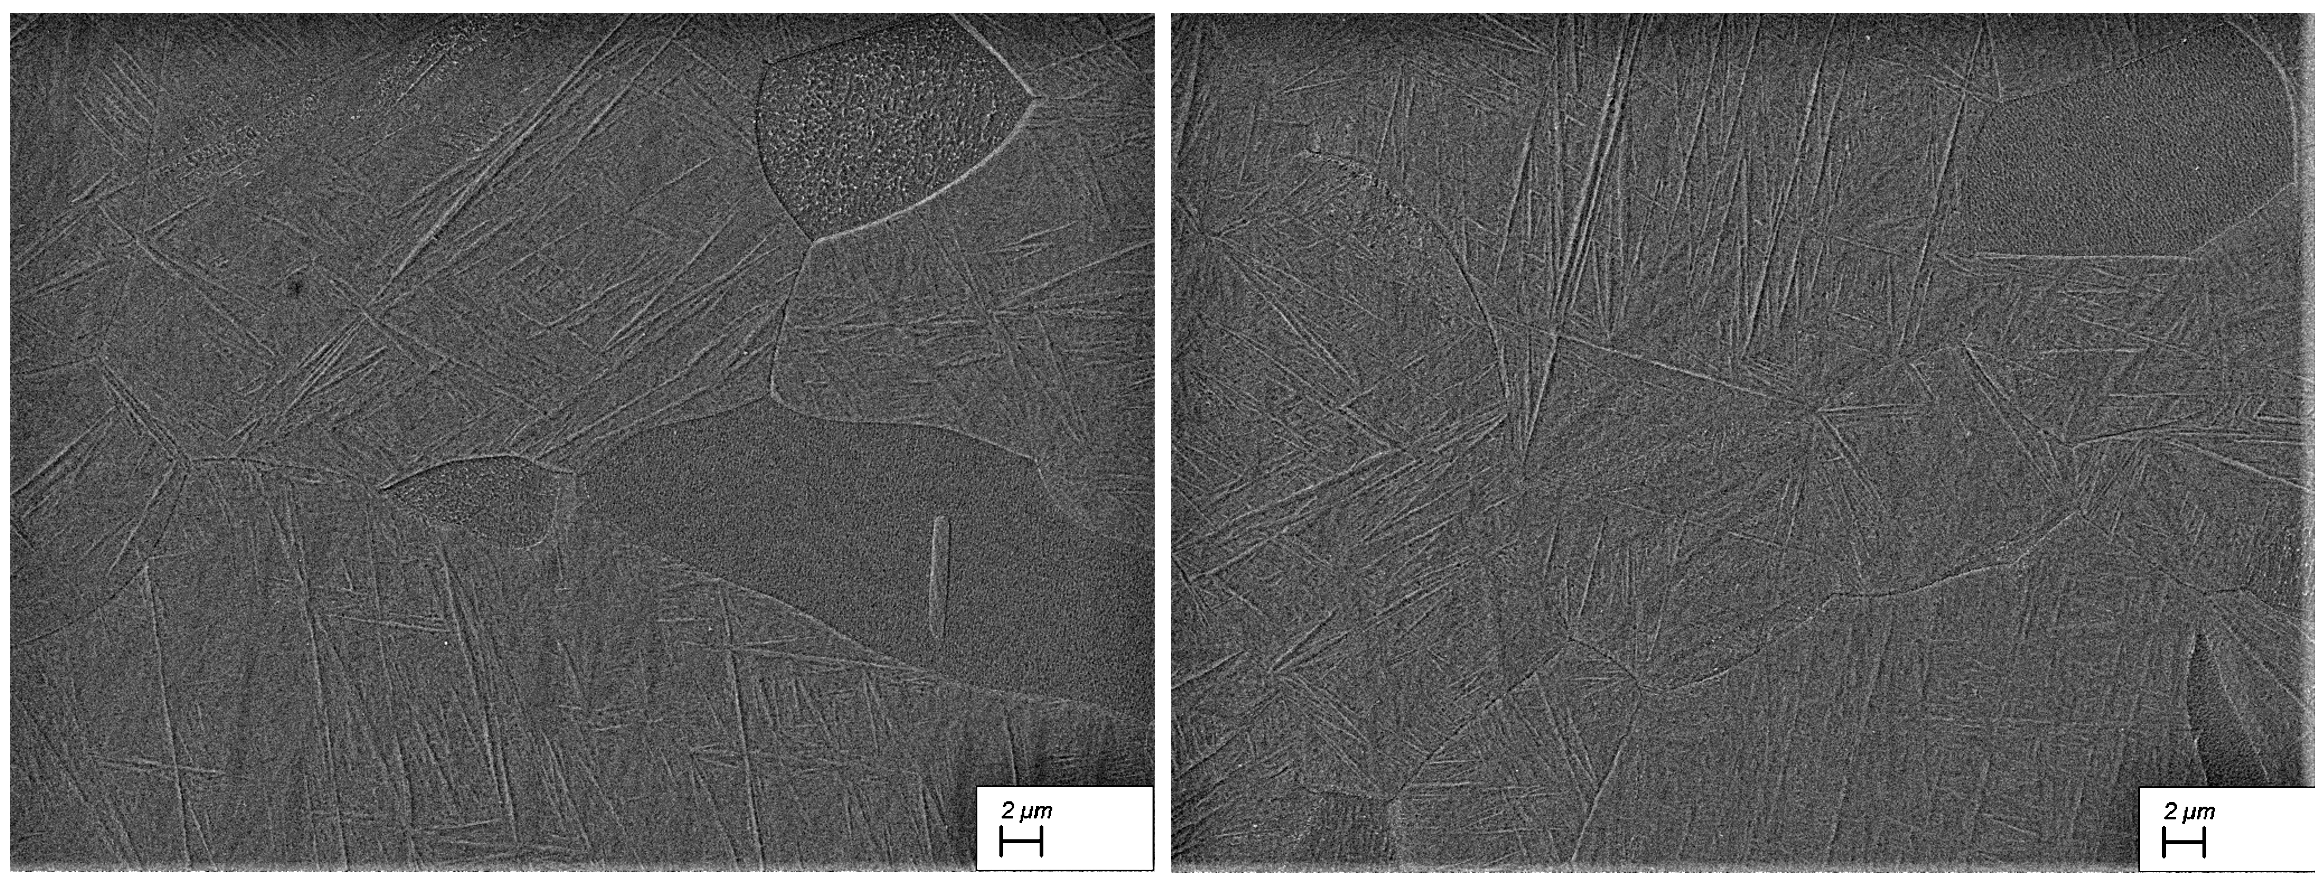
\includegraphics[width=1.0\linewidth]{./Bilder/Abbildung 26.png}
	\caption[Abbildung 26]{983$^\circ$C/1h/WQ + 610$^\circ$C/16min/AC, REM}
	\label{fig:abbildung-26}
\end{figure}

\begin{figure}
	\centering
	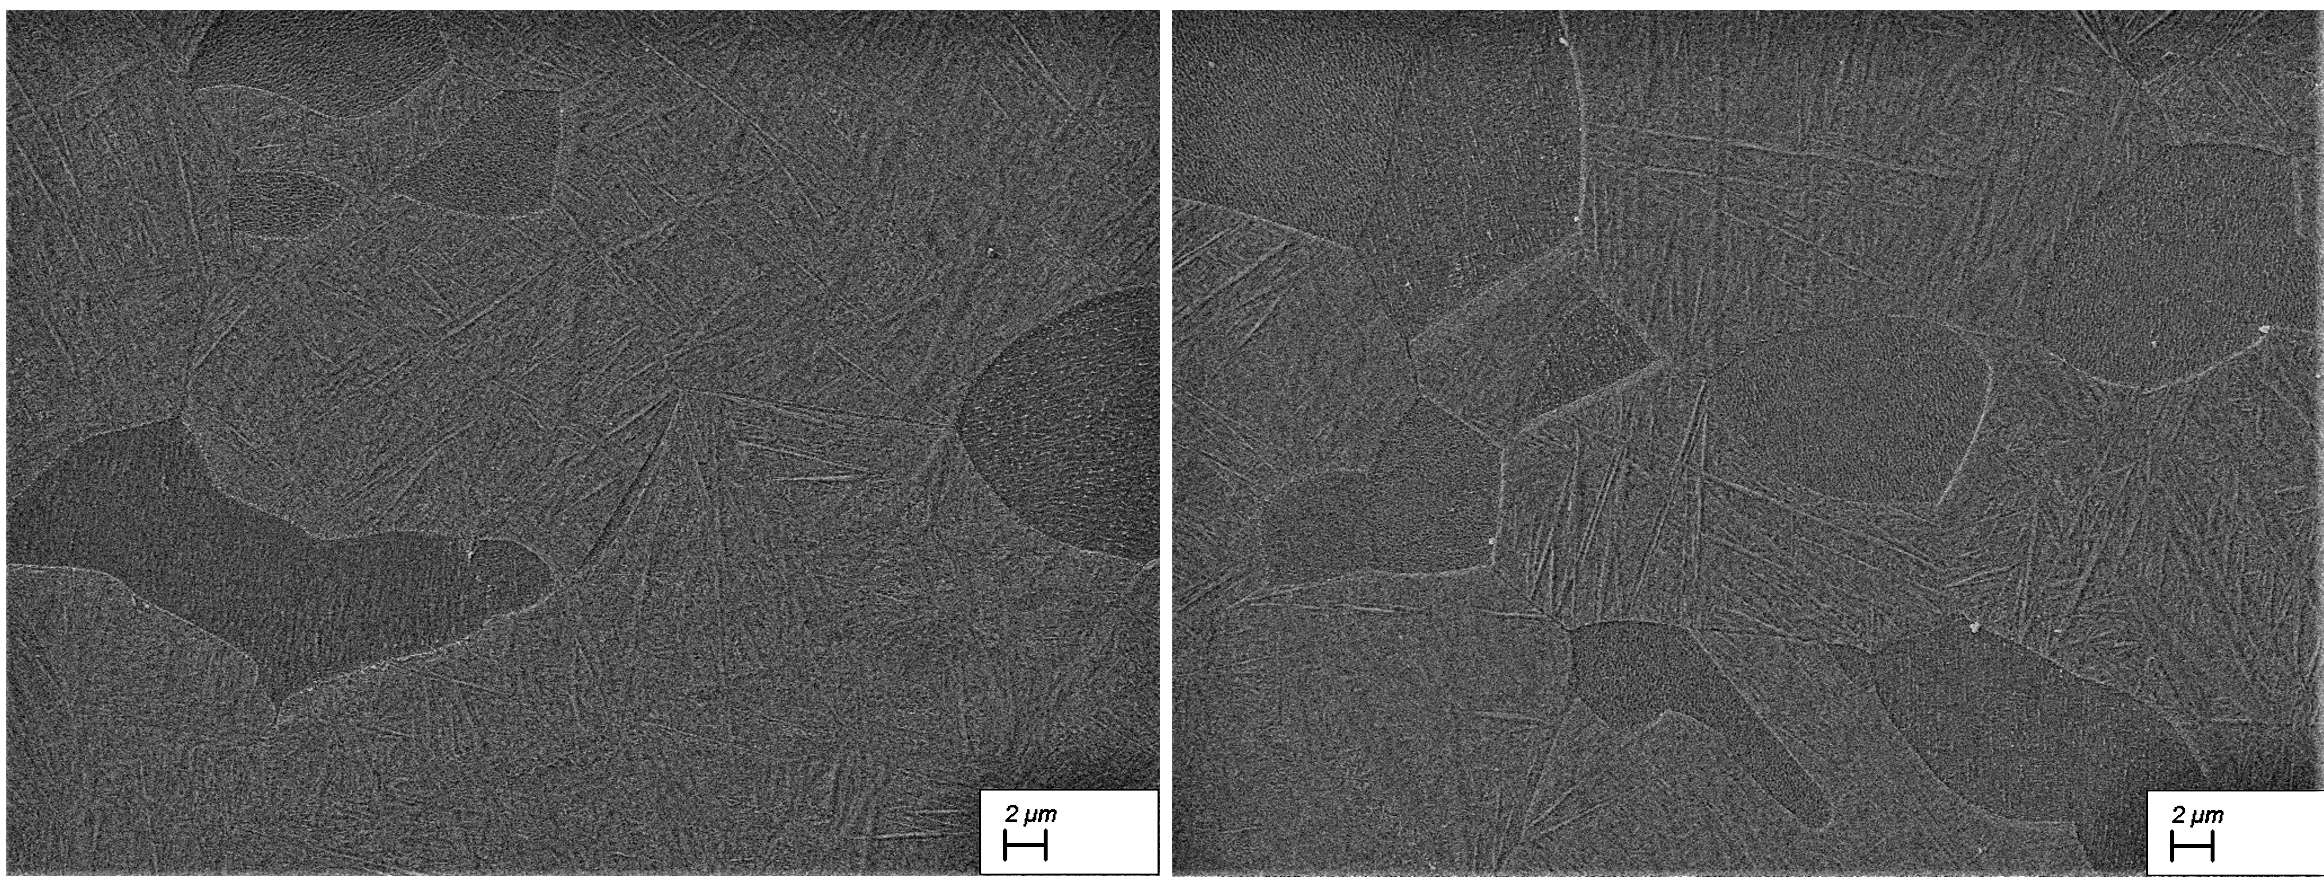
\includegraphics[width=1.0\linewidth]{./Bilder/Abbildung 27.png}
	\caption[Abbildung 27]{983$^\circ$C/1h/WQ + 610$^\circ$C/30min/AC, REM}
	\label{fig:abbildung-27}
\end{figure}

In den Abbildungen \ref{fig:abbildung-26} und \ref{fig:abbildung-27} ist zu erkennen, dass keine Veränderung in dem Gefüge im Vergleich zum vorherigen Schritt feststellbar ist. Es kann davon ausgegangen werden, dass der geplante Martensitzerfall nicht stattgefunden hat.

Die Ergebnisse der Härteprüfung nach diesem zweiten Schritt sind in Tabelle \ref{Tabelle 9} aufgeführt.

\begin{table}
	\centering
	\begin{tabular}{|c|c|}
		\hline 
		Probe & Härte in HV \\ 
		\hline 
		983$^\circ$C/1h/WQ + 610$^\circ$C/16min/AC & 405 \\ 
		\hline 
		983$^\circ$C/1h/WQ + 610$^\circ$C/30min/AC & 400 \\ 
		\hline 
	\end{tabular} 
	\caption{Ergebnisse der Härteprüfung nach der zweiten Wärmebehandlung, $\alpha_p$ - $\alpha'$ Gefüge}
	\label{Tabelle 9}
\end{table}

Es ist zu erkennen, dass auch die Härte unverändert im Vergleich zum vorherigen Schritt blieb.

(ZB)

\paragraph{Glühen und Abschrecken}
Nach dem Abschrecken hat sich die komplette $\beta$-Phase wie erwartet martensitisch umgewandelt. Die Bildung von den Martensit-Nadeln verfeinert das Gefüge. Das hat dazu geführt, dass sich die härte dieser Proben von 333 auf 405 HV10 gestigen ist. Duktilität ?
\paragraph{Anlassen} Nach dem Anlassen hat sich festgestellt, dass Martensit nicht zerfallen konnte. Das ist wahrscheinlich darauf zurückzuführen, dass die haltezeit , 30 min, nicht ausreichend für die Umwandlung der Martensitnadeln in  $\beta$ + $\alpha$ war bzw. war diese Transformation bei 610$^\circ$C so langsam, dass sie innerhalb von 30 min nicht stattfinden konnte.
Deshalb waren keine Änderungen im Gefüge im Vergleich zu dem ersten Schritt  festzustellen. Härte ?

